%
%
\documentclass[10pt,a4paper,oneside]{book}

%Hello there. Don't know what to do?
	%Search for the %? or \fixme and fix/add stuff.
	%Check zapiski 2007, your notes and your memory and fix/add stuff
	%kul knjige imajo quote na začetku poglavij
%
%lol, windows newline bug poje to vrsto včasih :P
%\documentclass[10pt,a4paper,oneside]{book}

\usepackage[slovene]{babel}
\usepackage[utf8x]{inputenc}
\usepackage[fleqn]{amsmath}%fleqn - levo zamaknjene enačbe
\usepackage{amsfonts}
\usepackage{amssymb}
\usepackage{makeidx}
\usepackage{graphicx}
\usepackage[x11names, rgb]{xcolor}
\usepackage{tikz}
\usetikzlibrary{calc,automata,snakes,arrows,shapes,decorations.text,positioning,shapes.arrows,chains}

\usepackage{torstyle}
%?this feels too much like CSS hacks :(
%torstlye predloge:
%Definicija \Def{}
%Primer \Primer{}
%Prirejen itemize \begin{items}
\hypersetup{pdftitle={Teoretične osnove računalništva}}

\begin{document}
\begin{titlepage}
\begin{center}
%looks useful
%{\resizebox{15cm}{!}{Teoretične osnove računalništva}}\\[5pt]
\ \\[1cm]
{\Huge\bf Teoretične osnove računalništva}\\[1cm]
{\huge \today}\ \\[1.5cm]
%{\LARGE Zapiski predavanj 2010/2011}\\[15pt]%Odkar sem dodal kontekstno-odvisne in linearne, to ni več to :P
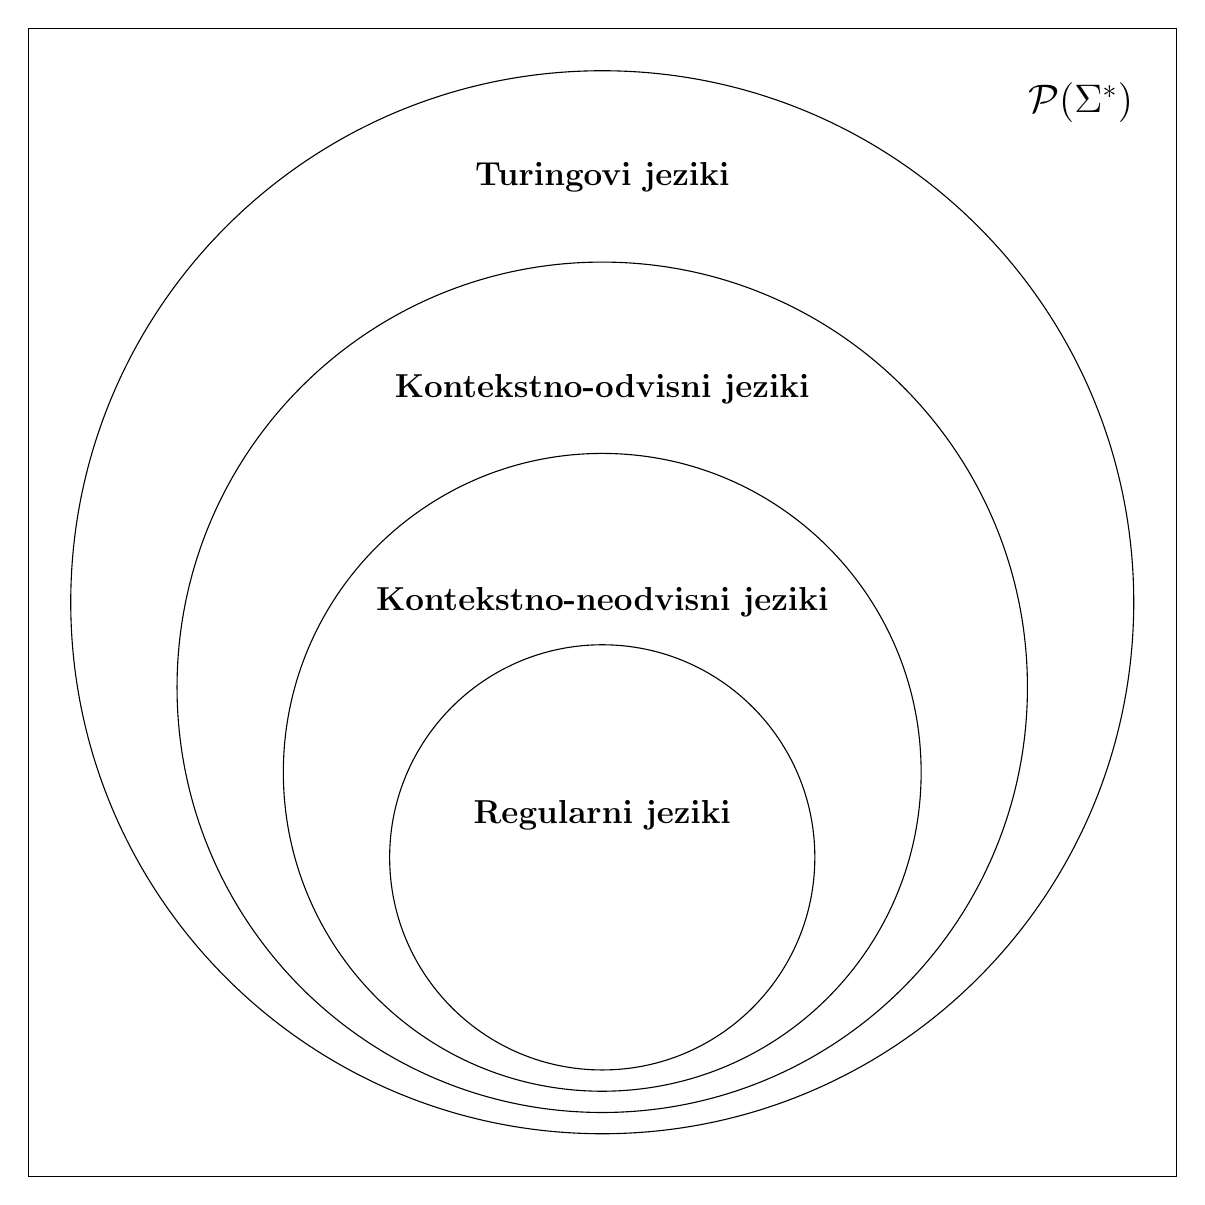
\begin{tikzpicture}[scale=1.35]
	\draw (-5.4cm,-5.4cm) rectangle (5.4cm,5.4cm);
	\node at (4.5cm,4.7cm) {\Large $\mathcal{P}(\Sigma^*)$};%sva šla vprašat... ker \Sigma^* znajo že RJ opisat, samo ne vseh možnih ;)

	\draw (0cm,0cm) circle (5cm);
	\node at (0,4cm) {\large\bf {Turingovi jeziki}};

	\draw (0cm,-0.8cm) circle (4cm);
	\node at (0,2cm) {\large\bf {Kontekstno-odvisni jeziki}};

	\draw (0cm,-1.6cm) circle (3cm);
	\node at (0,0cm) {\large\bf {Kontekstno-neodvisni jeziki}};

	\draw (0cm,-2.4cm) circle (2cm);
	\node at (0,-2cm) {\large\bf {Regularni jeziki}};
\end{tikzpicture}

\vfill
\parbox{7.5cm}{
\begin{center}

\includegraphics[width=0.15\textwidth]{./CC}\\[6pt]

This work is licensed under a Creative Commons Attribution-NonCommercial-ShareAlike 3.0 Unported License
\end{center}
}

\end{center}
\end{titlepage}
\tableofcontents
\pagebreak
%\newpage

\chap{Vaja 1 (4. 3. 2011)}
\sect{Turingovi stroji}

Turingov stroj se je uveljavil kot uporaben in preprost model računanja, ki zna izračunati vse kar se izračunati da (pod pogojem, da Church-Turingova teza drži). Alan Turing je svoj stroj izpeljal iz razmišljanja o tem, kako človek rešuje miselne probleme na papir. Pri tem je izbral tri sestavne dele:
\begin{items}
\item Nadzorno enoto (glava)
\item Čitalno okno (roka in vid)
\item Trak (papir)
\end{items}
V postopku formalizacije, pa je zaradi večje preprostosti, zahteval še, da je stroj sestavljen iz končno mnogo elementov, ter da deluje v diskretnih korakih.%?končno mnogo elementov? na kaj to cilja?
\ \\
\begin{center}
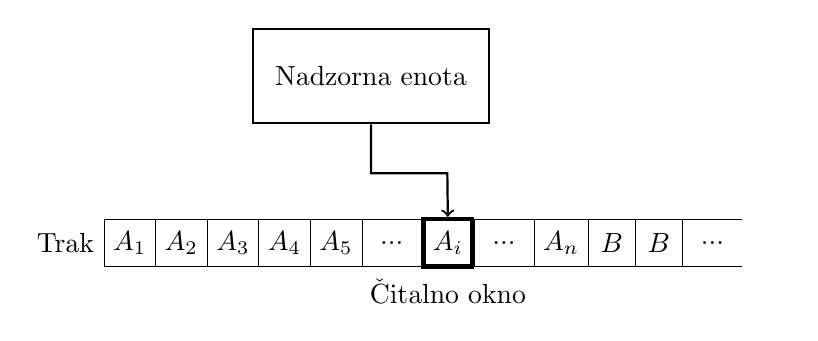
\begin{tikzpicture}[start chain, node distance=-0.075mm, thick, cell/.style={draw, very thin, on chain, minimum size=0.6cm}]
	\node (Trak) [on chain] {Trak};
	\foreach \x in {1,2,...,5} {
		\node ({A\x}) [cell] {$A_{\x}$};
	}
	\node ({Ad1}) [cell] {\ ...\ \ };
	\node ({Ai}) [cell, ultra thick] {$A_i$};
	\node ({Ad2}) [cell] {\ ...\ \ };
	\node ({An}) [cell] {$A_n$};
	\node ({Ab1}) [cell] {$B$};
	\node ({Ab2}) [cell] {$B$};
	\node ({Ad3}) [cell] {\ ...\ \ };
	\node ({end}) [cell, draw=white] {};

	%?must be a better way, zadnja črta niti ni naravnost
	\node (ne) at (110bp, 60bp) [draw, minimum height=1.2cm, minimum width=3cm]  {Nadzorna enota};
	\draw (ne.south) -- (110bp, 25bp) -- (137.5bp, 25bp) [->] to (Ai.north);
	\node [below] at (Ai.south) {Čitalno okno};
\end{tikzpicture}
\end{center}

\Def{Turingov stroj je definiran kot sedmerka $M=\langle Q, \Sigma, \Gamma, \delta, q_0, B, F \rangle $, kjer je:
\begin{items}
	\item $Q$ končna množica stanj
	\item $\Sigma$ končna množica vhodnih simbolov, $Q \cap \Sigma = \emptyset$
	\item $\Gamma$ končna množica tračnih simbolov, $\Sigma \subset \Gamma$
	\item $\delta$ funkcija prehodov: $Q \times \Gamma \rightarrow Q \times \Gamma \times \{L,D\}$,\\ kjer $L$ in $D$ označujeta premik levo ali desno
	\item $q_0$ začetno stanje, $q_0 \in Q$
	\item $B$ prazen simbol, $B \in \Gamma$
	\item $F$ množica končnih stanj, $F \subseteq Q$ 
\end{items}}
Stroj deluje tako, da v vsakem koraku opravi naslednje:
\begin{items}
	\item preide v neko stanje
	\item zapiše nov simbol v celico, ki je pod oknom
	\item okno premakne eno celico levo ali desno
\end{items}

\subsect{Trenutni opis}
\Def{$TO = \Gamma^* \times Q \times \Gamma^*$ je množica vseh trenutnih opisov.\\
Nek trenutni opis $\langle \alpha_1, q, \alpha_2 \rangle$, ali krajše $\alpha_1\ q\ \alpha_2$ opisuje konfiguracijo Turingovega stroja.
\br
\fixme naredi bolj formalen zapis!

\chap{Vaja 2 (7. 3. 2011)}
\sect{Turingovi stroji - nadaljevanje}

\pagebreak

\br
\pagebreak
\br

\begin{center}
\begin{tikzpicture}[start chain, node distance=-0.075mm, thick, cell/.style={draw, very thin, on chain, minimum size=0.6cm}]
	\node ({alpha1}) [cell, minimum width=4cm] {$\alpha_1$};
	\node ({Ai}) [cell, ultra thick] {};
	\node ({alpha2}) [cell, minimum width=3.5cm] {$\alpha_2$\ \ \ };
	%\node ({Ad2}) [cell] {};
	\node ({Ab1}) [cell] {$B$};
	\node ({Ab2}) [cell] {$B$};
	\node ({Ad3}) [cell] {\ ...\ \ };
	\node ({end}) [cell, draw=white] {};

	%?must be a better way, zadnja črta niti ni naravnost
	\node (ne) at (50bp, 60bp) [draw, minimum width=2cm, minimum height=1.2cm]  {$q$};
	\draw (ne.south) -- (50bp, 25bp) -- (66bp, 25bp) [->] to (Ai.north);
	%\node [below, minimum width=4cm] at (alpha1.south) {$\alpha_1$};
	%\node [below, minimum width=4cm] at (alpha2.south) {$\alpha_2$\ \ \ \ };
\end{tikzpicture}
\end{center}
\br
Čitalno okno je nad prvim znakom niza $\alpha_2$, iz tega lahko razberemo:
\begin{items}
	\item če je $\alpha_1 = \varepsilon$, je okno skrajno levo
	\item če je $\alpha_2 = \varepsilon$, je okno nad $B$ in so naprej sami $B$-ji
\end{items}}

\subsect{Relacija $\vdash$}
\Def{Če sta $u,v$ trenutna opisa iz množice $TO$, ter $v$ neposredno sledi iz $u$ v enem koraku Turingovega stroja, tedaj pišemo $u \vdash v$.
\br
Naj bo $x_1 \dots x_{i-1}\ q\ x_i \dots x_n$ trenutni opis:
\begin{items}
\item če je $\delta(q,x_i) = \langle p,Y,D \rangle$:\\
$x_1 \dots x_{i-1}\ q\ x_i \dots x_n \vdash x_1 \dots x_{i-1}\ Y\ p\ x_{i+1} \dots x_n$
\item če je $\delta(q,x_i) = \langle p,Y,L \rangle$: 
	\begin{items}
	\item če je okno na robu ($i=1$), se Turingov stroj ustavi, ker je trak na levi omejen.
	\item če okno ni na robu ($i>1$), potem: $x_1 \dots x_{i-2} x_{i-1}\ q\ x_i \dots x_n \vdash x_1 \dots\ x_{i-2} p\ x_{i-1}\ Y\ x_{i+1} \dots x_n$
	\end{items}
\end{items}}
Imamo pa tudi posplošeno relacijo $u \vdash^* v$, ki pove, da trenutni opis $v$ sledi iz $u$ v enem ali večih korakih.
\Def{$u \vdash^* v$, če obstaja tako zaporedje $x_i, (i \in [0, 1, \dots, k], k \geq 0)$, da velja $u=x_0, v=x_k$ in $x_0 \vdash x_1 \wedge x_1 \vdash x_2 \wedge \dots \wedge x_{k-1} \vdash x_k$
\br
Torej, trenutni opis $v$ sledi iz $u$, v $k$ korakih Turingovega stroja.}
\sect{Jezik Turingovega stroja}
\Def{Jezik Turingovega stroja je:
\begin{equation*}
L(M) = \{ w\ |\ w \in \Sigma^* \wedge \varepsilon\ q_0\ w \vdash^*\alpha_1\ q_F\ \alpha_2 \wedge \alpha_1,\alpha_2 \in \Gamma^*, q_F \in F \}
\end{equation*}
}
Z besedami to pomeni, da je jezik Turingovega stroja množica besed, ki če jih damo na vhod stroja, povzročijo, da se ta v končno mnogo korakih znajde v končnem stanju.
\ \\
\begin{center}
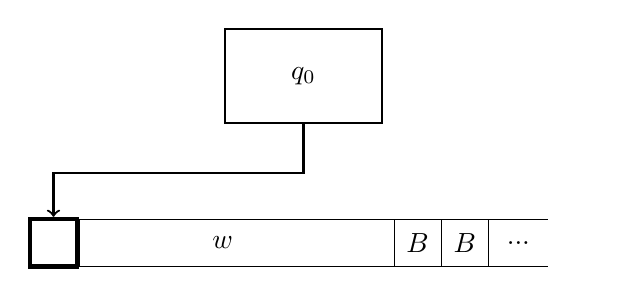
\begin{tikzpicture}[start chain, node distance=-0.075mm, thick, cell/.style={draw, very thin, on chain, minimum size=0.6cm}]
	\node ({Ai}) [cell, ultra thick] {};
	\node ({w}) [cell, minimum width=4cm] {$w$\ \ \ \ };
	\node ({Ab1}) [cell] {$B$};
	\node ({Ab2}) [cell] {$B$};
	\node ({Ad}) [cell] {\ ...\ \ };
	\node ({end}) [cell, draw=white] {};

	%?must be a better way, zadnja črta niti ni naravnost
	\node (ne) at (90bp, 60bp) [draw, minimum width=2cm, minimum height=1.2cm]  {$q_0$};
	\draw (ne.south) -- (90bp, 25bp) -- (0bp, 25bp) [->] to (Ai.north);
\end{tikzpicture}
\br
Začetna konfiguracija Turingovega stroja.
\end{center}
\Def{Jezik $L$ je Turingov jezik, če obstaja Turingov stroj $M$, tak, da je $L = L(M)$.}
\subsect{Ugotavljanje pripadnosti besed Turingovemu jeziku}
Pri vprašanju ali je neka beseda v jeziku, Turingove jezike ločimo na:
\begin{items}
\item Odločljive - obstaja algoritem, s katerim se lahko za poljubno besedo odločimo, ali pripada jeziku.
\item Neodločljive - v splošnem ni algoritma, ki bi za poljubno vhodno besedo z DA ali NE odgovoril na vprašanje pripadnosti.
	\begin{items}
	\item če je odgovor DA, to ugotovimo v nekem končnem številu korakov.
	\item če je odgovor NE, pa ni nujno, da se bo stroj kdaj ustavil.
	\end{items}
\end{items}

%?\fixme - vennov diagram beseda w znotraj L kroga... pomojm ne rabmo :P

%?where does this go?
%Terminologija: re (recursively enumerable, Turing recognizable)%?semi-decidable? 
%Rekurzivni jezik (decidable)%?where does this go?

\fixme - vennov diagram odločljivi jeziki znotraj Turingovih?

\Primer{Zapiši Turingov stroj, ki sprejema jezik $L=\{0^n 1^n | n \geq 1\}$\\
	Skica izvajanja stroja:
	\begin{items}
	\item $0^{n}1^{n}$ - vhodna beseda
	\item $X0^{n-1}1^{n}$ - zamenjamo najbolj levo $0$ z $X$
	\item $X0^{n-1}Y1^{n-1}$ - premaknemo okno desno do najbolj leve $1$ in jo zamenjamo z $Y$
	\item $XX0^{n-2}Y1^{n-1}$\\ 
		$XX0^{n-2}YY1^{n-2}$ - ponovimo in vidimo, da bomo niz sprejeli, če je prave oblike.
	\end{items}
	Turingov stroj zapišemo kot $M=\langle Q,\Sigma,\Gamma,\delta,q_0,B,F \rangle$:
	\begin{items}
    \item $Q=\{ q_0,q_1,q_2,q_3,q_4 \}$
    \item $\Sigma = \{ 0,1 \}$
    \item $\Gamma = \{ 0,1,B,X,Y \}$
    \item $F = \{ q_4 \}$
    \item $\delta$ bomo definirali s tabelo
	\end{items}

    Pomen stanj:
    \begin{items}
    \item $q_0$ - začetno stanje in stanje pred zamenjavo 0 z X
    \item $q_1$ - premikanje desno do 1
    \item $q_2$ - zamenjava 1 z Y in premikanje levo do X
    \item $q_3$ - najde X in se premik desno
    \item $q_4$ - končno stanje
    \end{items}

    Tabela prehajanja stanj:\\
	\begin{center}
    \begin{tabular}{ c | c c c c c}
	& 0 & 1 & B & X & Y\\ \hline
	$x_0$& $\langle q_1,X,D\rangle$ & -- & -- & $\langle q_3,Y,D\rangle$ & --\\
	$x_1$& $\langle q_1,0,D\rangle$ & $\langle q_2,Y,L\rangle$ & -- & $\langle q_1,Y,D\rangle$ & --\\
	$x_2$& $\langle q_2,0,D\rangle$ & -- & $\langle q_0,X,D\rangle$ & $\langle q_2,Y,L\rangle$ & --\\
	$x_3$& -- & -- & -- & $\langle q_3,Y,D\rangle$ & $\langle q_4,B,D\rangle$\\
	$x_4$& -- & -- & -- & -- & --\\
	\end{tabular}
	\end{center}
	\br
	Izvajanje stroja s trenutnimi opisi:
	\[ q_0 0011 \vdash X q_1 011 \vdash X 0 q_1 11 \vdash X q_2 0 Y 1 \vdash \dots \]
}
%?zapiski 2007 imajo tu še nekaj o turingovih jezikih
\subsect{Turingov stroj kot računalnik funkcij}
Imamo Turingov stroj, ki ima na traku neko število ničel, ki predstavljajo pozitivna naravna števila, ločena z enicami:
%	\[ 0^{i_1} 1 0^{i_2} 1  \dots 1 0^{i_k} \]
%?skupine ničel so i_1, i_2, ..., kjer so i naravna števila (mjbi i+1 ničel)  
\ \\
\begin{center}
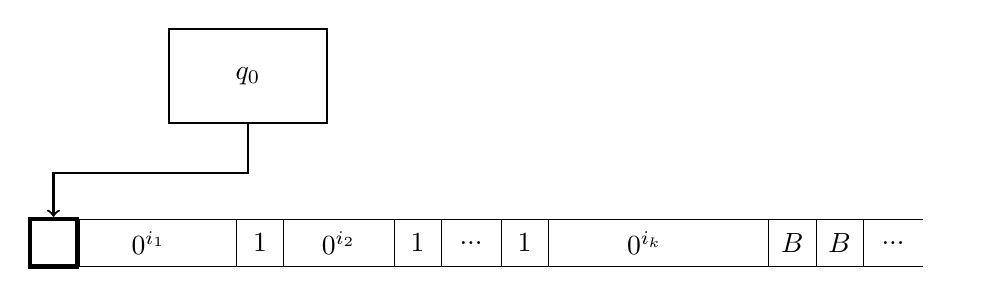
\begin{tikzpicture}[start chain, node distance=-0.075mm, thick, cell/.style={draw, very thin, on chain, minimum size=0.6cm}]
	\node ({Ai}) [cell, ultra thick] {};
	\node ({A0}) [cell, minimum width=2cm] {$0^{i_1}$\ \ \ };
	\node ({Ab1}) [cell] {$1$};
	\node ({A1}) [cell, minimum width=1.4cm] {$0^{i_2}$};
	\node ({Ab1}) [cell] {$1$};
	\node ({Ad1}) [cell] {\ ...\ \ };
	\node ({Ab1}) [cell] {$1$};
	\node ({A1}) [cell, minimum width=2.8cm] {$0^{i_k}$\ \ \ \ };
	\node ({Ab1}) [cell] {$B$};
	\node ({Ab1}) [cell] {$B$};
	\node ({Ad2}) [cell] {\ ...\ \ };
	\node ({end}) [cell, draw=white] {};

	%?must be a better way, zadnja črta niti ni naravnost
	\node (ne) at (70bp, 60bp) [draw, minimum width=2cm, minimum height=1.2cm]  {$q_0$};
	\draw (ne.south) -- (70bp, 25bp) -- (0bp, 25bp) [->] to (Ai.north);
\end{tikzpicture}
\end{center}
Recimo, da se stroj po nekem številu korakov ustavi in ima na traku skupino ničel $0^m$, na levi in desni strani skupine pa same $B$-je. S tem je stroj morda izračunal neko funkcijo:
	\[ f^{(k)}:\mathbb{N}_+^k \rightarrow \mathbb{N}_+ \mbox{\ \ oz. \ \ } f(i_1, i_2, \dots, i_k) = m \]
%?\fixme - slika TS s skupino ničel na traku\br... pomojm ne rabmo :P
Funkcija $f$ ni nujno definirana za vsako $k$-terico iz $\mathbb{N}_+^k$, torej je parcialna funkcija, kadar pa je definirana povsod, pravimo da je totalna. Stroj se pri nedefiniranih $k$-tericah pač na neki točki ustavi in pri tem na traku ne pusti le ene skupine ničel, ali pa se sploh ne ustavi.
Isti turingov stroj hkrati računa več funkcij: $f^{(1)}, f^{(2)}, \dots f^{(k)}$.%?računa ali "lahko računa".. ne štekam ubistvu čist

\subsubsection{Parcialna rekurzivna funkcija}
\Def{Vsaka funkcija $f^{(k)}:\mathbb{N}_+^k \rightarrow \mathbb{N}$, ki jo lahko izračuna nek Turingov stroj, je parcialna rekurzivna funkcija. Če je $f^{(k)}$ definirana za vse $k$-terice, jo imenujemo totalna rekurzivna funkcija (včasih samo rekurzivna funkcija)}
Vse običajne aritmetične funkcije so parcialne ali celo totalne rekurzivne funkcije. V primerih si bomo pogledali nekaj primerov, tu pa jih nekaj naštejmo: $m+n,\ m*n,\ n!,\ 2^n,\ \lceil \log(n) \rceil,\ m^n,\ \dots$.
%so najdl primer, ki ne spada sem z diagonalizacijo
%na začetku so gledali totalne... pa so vidl da morajo parcialne
\begin{primeri}
\item
    Ali je $f(m,n)=m+n$ (parcialno) rekurzivna?\\
    Skica stroja, ki računa $m+n$:
    \begin{items}
    \item $0^m 1 0^m$ - vhodna beseda
    \item $B0^{m-1} 1 0^m$ - izbriši prvo ničlo
    \item $B0^{m+n}$ - premakni se do 1 in jo zamenjaj z 0
    \end{items}%?DN naredi cel stroj
\item
    Ali je $f(m,n)=m*n$ (parcialno) rekurzivna?\\
    Skica stroja, ki računa $m*n$:
    \begin{items}
    \item $0^m 1 0^n$ - vhodna beseda
    \item $0^m 1 0^n 1$ - premakni se na konec in zapiši 1 (ločnica za rezultat)
    \item $B 0^{m-1} 1 0^n 1$ - premakni se na začetek in izbriši 0
    \item $B 0^{m-1} 1 0^m 1 0^n$ - prekopiraj $n$ ničel za ločnico (in ničle)
    \item $B^{m} 1 0^m 1 0^{m*n}$ - ponavljaj tadva koraka, dokler ni več ničel pred prvo 1
    \item $B^{m+n+2}0^{m*n}$ - izbriši del, ki ne spada v rezultat 
    \end{items}%?naredi cel stroj
\end{primeri}

\subsect{Lažja konstrukcija Turingovih strojev}
Obstaja nekaj tehnik, ki poenostavijo in pohitrijo sestavljanje Turingovih strojev.%tu itak mislimo funkcije delta
\subsubsection{Nadzorna enota kot pomnilnik}
Vsako stanje stroja, je sestavljeno iz dveh delov -- stanja avtomata, ter shrambe za tračne znake. Novo množico stanj zapišemo kot $Q=K\times\Gamma$, kjer je $K$ stara množica stanj in $\Gamma$ tračna abeceda.
\Primer{Sestavi Turingov stroj za razpoznavanje besed, pri katerih se prvi znak ne ponovi:\\
	Stroj $M=\langle Q,\Sigma,\Gamma,\delta,q_0,B,F \rangle$ zapišemo kot:
	\begin{items}
	\item $M=\langle Q, \{0,1\}, \{0,1,B\}, \delta, \langle q_0, B \rangle, B, F \rangle$
	\item $Q=\{ q_0, q_1 \} \times \{0,1,B\} = \{ \langle q_0, 0\rangle , \langle q_0, 1\rangle , \langle q_0, B\rangle , \langle q_1, 0\rangle , \langle q_1, 1\rangle , \langle q_1, B\rangle\} $
	\item $F=\{ \langle q_1, B \rangle \}$
	\item $\delta$ zapišemo kot:
		\begin{items}
		\item Shrani prvi znak besede v stanje stroja:\\
			$\delta(\langle q_0, B\rangle, 0) = \langle\langle q_1, 0 \rangle, 0, D\rangle$\\
			$\delta(\langle q_0, B\rangle, 1) = \langle\langle q_1, 1 \rangle, 1, D\rangle$
		\item Premakni okno v desno do prvega znaka, enakega shranjenemu:\\
			$\delta(\langle q_1, 0\rangle, 1) = \langle\langle q_1, 0 \rangle, 1, D\rangle$\\
			$\delta(\langle q_1, 1\rangle, 0) = \langle\langle q_1, 1 \rangle, 0, D\rangle$
		\item Če prebereš $B$, pojdi v končno stanje:\\
			$\delta(\langle q_1, 0\rangle, B) = \langle\langle q_1, B \rangle, karkoli \rangle$\\
			$\delta(\langle q_1, 1\rangle, B) = \langle\langle q_1, B \rangle, karkoli \rangle$
		\item Sicer se ustavi. To dosežemo tako, da ne definiramo prehodov:\\
			$\delta(\langle q_1, 0\rangle, 0)$ in $\delta(\langle q_1, 1\rangle, 1)$
		\end{items}
	\end{items}
}
\subsubsection{Večsledni trak}
Na traku imamo več kot eno sled, kar pomeni, da s traku beremo $k$-terice tračnih znakov, kar zapišemo kot: $\Gamma=\Gamma_1\times\Gamma_2\times\dots\times\Gamma_k$.
\Primer{Sestavi Turingov stroj, ki preveri, ali je vhodno število praštevilo.\\
	Skica stroja:
	\begin{items}
	\item Trak ima tri sledi:
		\begin{items}
		\item na prvi sledi je vhodno število
		\item na drugi sledi je števec, ki na začetku hrani število 2
		\item tretjo sled uporabimo za delovno sled, na začetku je lahko prazna.
		\end{items}
	\item Stroj deluje tako:
		\begin{items}
		\item prepiši število s prve sledi na tretjo sled
		\item odštevaj število iz druge sledi od števila na tretji sledi
		\item če se odštevanje konča z 0, se ustavi (ni praštevilo)
		\item sicer število na drugi sledi povečaj za 1
		\item če je število na drugi sledi enako tistemu na prvi, sprejmemo (je praštevilo)
		\item sicer, ponovimo postopek
		\end{items}
	\end{items}
}
\subsubsection{Prestavljanje vsebine traku}
Recimo, da bi s traku radi vzeli nekaj zaporednih znakov tako, kot da bi jih izrezali iz traku in nato trak zlepili nazaj skupaj, izrezane simbole pa bi si pri tem seveda radi nekako zapomnili. Tudi to metodo realiziramo s pomočjo shrambe za tračne simbole v nadzorni enoti, a moramo pri tem paziti, da je funkcija prehodov pravilno napisana.
\br\fixme slika "gube" na traku in slika nadzorne enote
\Primer{Sestavi Turingov stroj, ki premakne vsebino traku za 2 celici v desno.\\
	Skica stroja:
	\begin{items}
    \item $Q$ vsebuje stanja oblike: $\langle q, A_1, A_2 \rangle;\ q \in \{ q_1, q_2 \},\ A_1, A_2 \in \Gamma$
    \item $\Gamma$ poleg ostalih znakov, vsebuje še poseben znak $X$, ki označuje izpraznjeno celico na traku
	\item $F=\{ q_2 \}$
	\item $\delta$ zapišemo kot:
		\begin{items}
		\item Prva koraka -- zapomni si in izprazni prvi in drugi znak:\\
			$\delta(\langle q_1, B, B\rangle, A_1) = \langle\langle q_1, B, A_1 \rangle, X, D \rangle $\\
			$\delta(\langle q_1, B, A_1\rangle, A_2) = \langle\langle q_1, A_1, A_2 \rangle, X, D \rangle $
		\item Zapomni si nov znak in prvega iz shrambe zapiši na trak:\\
			$\delta(\langle q_1, A_i, A_{i+1}\rangle, A_{i+2}) = \langle\langle q_1, A_{i+1}, A_{i+2} \rangle, A_i, D \rangle $
		\item Zadnja koraka -- zapiši vsebino shrambe na trak:\\
			$\delta(\langle q_1, A_{n-1}, A_{n}\rangle, B) = \langle\langle q_1, A_{n}, B \rangle, A_{n-1}, D \rangle $\\
			$\delta(\langle q_1, A_{n}, B\rangle, B) = \langle\langle q_2, B, B \rangle, A_{n}, L \rangle $
		\end{items}
	\end{items}
}

%?\fixme ... tu je razlagal tisto neizračunljivo funkcijo nad matrikami. btw, @zidar: poglej tor2-dodatno.pdf - tam govori o preroku

\subsubsection{Podprogrami}
\fixme
%?Imamo neka posebna stanja, ki signalizirajo vhod in izhod iz podprograma%?je tu govoril o dveh strojih?


\end{document}